\documentclass[11pt]{article} % use larger type; default would be 10pt

\usepackage{graphicx}
\usepackage{amsmath}
\usepackage{fullpage}
\usepackage[parfill]{parskip}

\title{ME 597 Lab 3 Report}
\author{Iain Peet \and Andrei Danaila \and Kevin Kyeong \and Abdel Hamid \and Douche Salam}

\begin{document}
\maketitle

\clearpage

\section{Introduction}
In this lab exercise the Potential Fields and Wavefront methods are implemented for planning the robot's path around a know obstacle grid map. The methods produce a path that the robot can follow to travel from a given start position towards a predefined goal while avoiding known obstacles.

\section{Potential Fields Path Planning}
\subsection{Standard Method}
The potential field method defines 

\subsection{Steering}
The robot follows the planned path by steering towards the angle of steepest decent in the potential field map. This allows the robot to calculate the steering angle from any position on the map where the gradient is defined, which is essentially in every free cell in the grid.

Alternatively, we can define waypoints along the path of steepest decent and use the Stanley non-linear steering controller to follow it, but this would be more error prone due to the robot's poor steering which makes it more likely to deviate significantly from the intended path.

\subsection{Results and Observations}
The wavefront method for path planning successfully plotted a map through the obstacles.
The downside of this algorithm was noticed as resulting in substatial increase in steering controller usage
when compared to the wavefront planning method. This was caused to the large number of varying
gradients that the controller tried to follow on its way to the goal.

\begin{figure}[hbt]
 \centering
 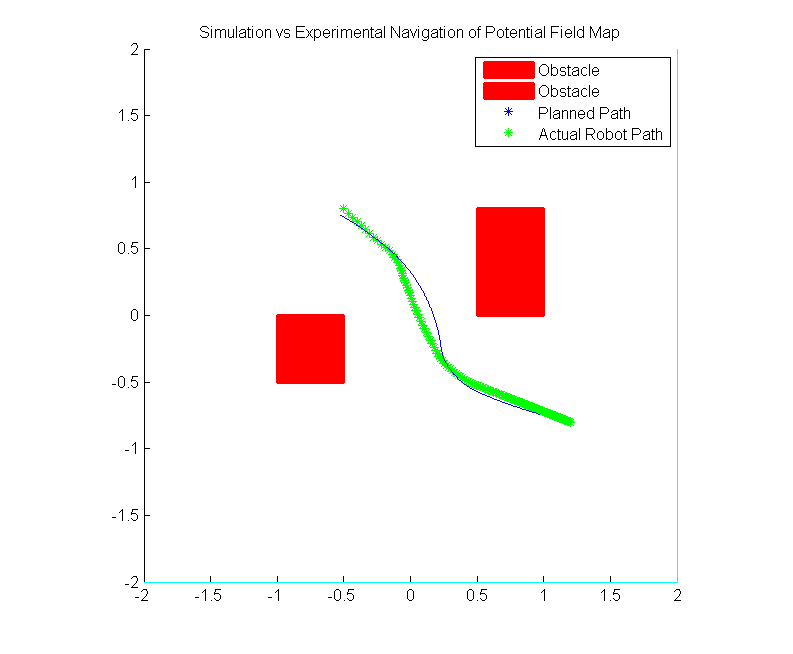
\includegraphics[scale=0.80]{potentialFieldMapNavigation.png}
 \caption{Traversed path through the obstacle map using the potential field algorithm.}
 \label{potFieldMap}
\end{figure}

From \ref{potFieldMap} it is noticed how even though the simulation predicted a sharper turn, 
the robot steering controller could not follow it. Since the robot was not able to perform 
such sharp turns, the volume of the each obstacle was increased in simulation as to provide an artificial
margin of safety to compensate for the lack of steering bandwidth.

\begin{figure}[hbt]
 \centering
 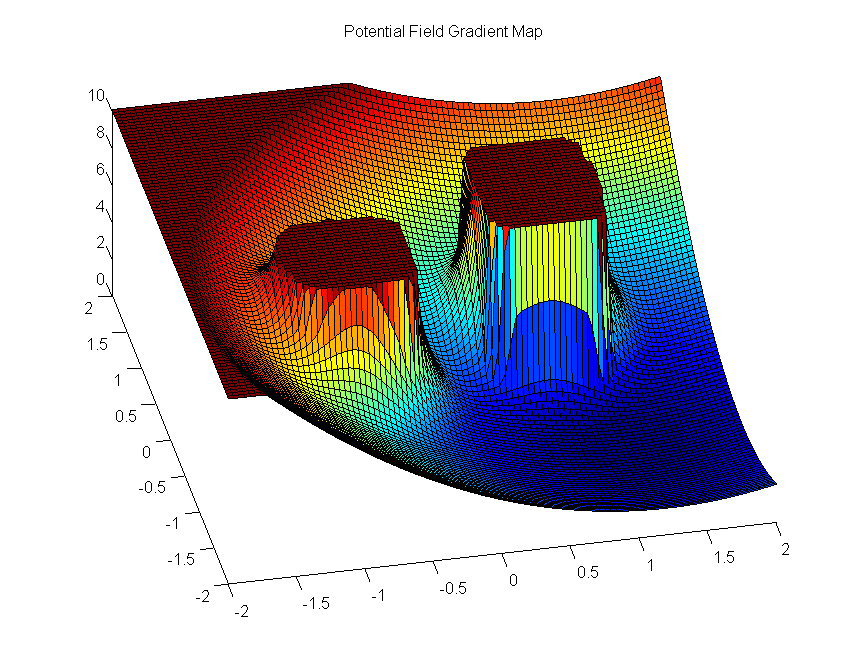
\includegraphics[scale=0.60]{Potential_Field_Surf_Plot.png}
 \caption{Potential field map surface plot.}
 \label{potField_Surf}
\end{figure}


\subsection{Extended Potential Fields}
\section{Wavefront Path Planning}


\end{document}


